\documentclass[11pt]{article}

\usepackage[margin=1in]{geometry}
\usepackage{amsmath,amssymb}
\usepackage{booktabs}
\usepackage{graphicx}
\usepackage{longtable}
\usepackage[dvipsnames]{xcolor}
\usepackage[colorlinks=true,linkcolor=NavyBlue,urlcolor=NavyBlue]{hyperref}
\usepackage{enumitem}
\usepackage{caption}
\usepackage{fancyhdr}
\usepackage{titlesec}

\captionsetup{font=small,labelfont=bf}
\setlist{itemsep=2pt,parsep=0pt,topsep=3pt}
\titlespacing*{\section}{0pt}{14pt}{6pt}
\titlespacing*{\subsection}{0pt}{10pt}{4pt}

\pagestyle{fancy}
\fancyhf{}
\fancyhead[L]{\small STAT 638 Project 17 --- Bayesian Forecasting of Household Electricity Demand}
\fancyhead[R]{\small\thepage}
\renewcommand{\headrulewidth}{0.4pt}

\newcommand{\kwh}{\,\mathrm{kWh}}
\newcommand{\code}[1]{\texttt{\small #1}}

\title{\vspace{-1.2cm}\textbf{Bayesian Forecasting of Household Electricity Demand}\\[2pt]
\large Project 17 --- methods, modelling decisions, and obstacles}
\author{Technical working document}
\date{\today}

\begin{document}
\maketitle
\thispagestyle{fancy}

\begin{abstract}
\noindent
This document records what the project asks for, how the data were prepared, what
model was built and why, which algorithms were implemented to fit it, and --- at
equal length --- what went wrong along the way. Four years of one-minute
electricity measurements from a single French household are aggregated to
$1{,}417$ usable daily consumption totals and modelled with a Bayesian harmonic
regression carrying a linear trend, annual harmonics at period $365$ days,
day-of-week effects, and a heavy-tailed autoregressive error process. Inference
uses a purpose-built Gibbs sampler with Metropolis steps, validated against
simulated data with known truth. Seven specifications are compared by WAIC and,
more importantly, by genuinely held-out forecasts over a twelve-month test
period. Several conclusions reverse the choices that seemed obvious at the
outset: the log transform hurts rather than helps, an AR(2) error process is
favoured by WAIC but rejected out of sample, and a plain day-of-year
climatology still outperforms every fitted model at long horizons. The last of
these remains open and is documented as such.
\end{abstract}

\section{What the project asks}

\subsection{The brief}

The assignment supplies a dataset, mandates one component of the model, and
poses six questions. In its own terms: characterise temporal patterns in daily
household electricity consumption, and develop a Bayesian analysis usable for
predicting future daily demand.

The seasonal component is not a free choice. The model \emph{must} represent
annual seasonality with sine and cosine terms at period $365$ days, beginning
with the first harmonic, $\sin(2\pi t/365)$ and $\cos(2\pi t/365)$, and the
analysis must investigate whether adding the second harmonic,
$\sin(4\pi t/365)$ and $\cos(4\pi t/365)$, improves the representation.

\subsection{The six questions, and what each one forces into the model}

The questions read like prose but function as a specification. Each names a
term the model must contain and a posterior that must be reported.

{\small
\begin{longtable}{@{}p{0.29\textwidth}p{0.27\textwidth}p{0.38\textwidth}@{}}
\toprule
\textbf{Question} & \textbf{Required model term} & \textbf{Required output} \\
\midrule
\endfirsthead
\toprule
\textbf{Question} & \textbf{Required model term} & \textbf{Required output} \\
\midrule
\endhead
Q1. How does consumption vary over the study period?
& Nothing new; descriptive
& Series plot, summary statistics, variance decomposition by component \\[3pt]
Q2. Is there a long-term increase or decrease?
& Linear trend in $t$
& Posterior of the slope in $\kwh$/year and \%/year, with
  $\Pr(\text{slope}<0\mid\text{data})$ \\[3pt]
Q3. What annual pattern is present, and does harmonic 2 improve on harmonic 1?
& Harmonics (mandated)
& Amplitude and phase in $\kwh$; a defended comparison of $J{=}1$ against $J{=}2$ \\[3pt]
Q4. Are there systematic weekly patterns?
& Day-of-week effects
& Seven posterior deviations with intervals; is the weekend genuinely different? \\[3pt]
Q5. How accurately can demand be predicted, and how does uncertainty change with horizon?
& A serially correlated error process, plus honest validation
& Predictive interval width as a function of $h$; held-out accuracy and coverage \\[3pt]
Q6. Are there periods not adequately explained by the model?
& Nothing new, but requires posterior predictive checking
& A dated table of anomalies with interpretation \\
\bottomrule
\end{longtable}
}

Two consequences follow immediately. First, trend, harmonics, day-of-week
effects, and a correlated error term are all mandatory --- omit any one and a
question becomes unanswerable. Second, Q5 is the load-bearing question, and it
is the one that rules out the simplest error assumption: if errors were
independent, predictive uncertainty would be identical one day ahead and three
hundred days ahead, which is both false and exactly what the question probes.

\subsection{Why this is a Bayesian problem}

The word ``uncertainty'' appears three times in the brief. A frequentist could
fit this regression in one line. What the assignment wants is a posterior
distribution for every quantity and a full predictive distribution for every
future day, so that statements like ``the annual cycle swings
$16.2\kwh$/day, 95\% CI $[14.6, 17.7]$'' and ``there is a $77.5\%$ posterior
probability that consumption is declining'' are available directly rather than
through an appeal to asymptotics.

\section{The data}

\subsection{Provenance and physical form}

The UCI \emph{Individual Household Electric Power Consumption} dataset records
$2{,}075{,}259$ one-minute measurements from a house in Sceaux, about 7\,km
from Paris, between December 2006 and November 2010 (47 months). It was
donated by Georges H\'ebrail and Alice B\'erard of EDF R\&D, the French
national utility. This is \emph{one house}, not a grid --- a point that governs
how every conclusion must be worded.

\begin{sloppypar}
The file \code{household\_\allowbreak power\_\allowbreak consumption.txt} is
semicolon-delimited, roughly 127\,MB uncompressed, with nine columns:
\end{sloppypar}

\begin{center}
\small
\begin{tabular}{@{}clll@{}}
\toprule
\# & Column & Unit & Content \\
\midrule
1 & \code{Date} & dd/mm/yyyy & European format, day first \\
2 & \code{Time} & hh:mm:ss & Local time \\
3 & \code{Global\_active\_power} & kW & \textbf{The raw material}: mean real power that minute \\
4 & \code{Global\_reactive\_power} & kW & Reactive power; unused \\
5 & \code{Voltage} & V & Near 240; unused \\
6 & \code{Global\_intensity} & A & Nearly collinear with column 3; unused \\
7 & \code{Sub\_metering\_1} & Wh & Kitchen (dishwasher, oven, microwave) \\
8 & \code{Sub\_metering\_2} & Wh & Laundry (washer, drier, fridge, light) \\
9 & \code{Sub\_metering\_3} & Wh & Electric water heater and air conditioner \\
\bottomrule
\end{tabular}
\end{center}

The three sub-meters deliberately do not sum to the total; the remainder
(lighting, electronics, heating) is the bulk of consumption and is used here
only as a validation check.

\subsection{Four traps that silently corrupt the pipeline}

\begin{enumerate}[leftmargin=*]
\item \textbf{Missing values are the literal character \code{?}}, not blanks.
Without declaring it, every numeric column parses as text and daily totals
come out as garbage or raise errors.
\item \textbf{Dates are day-first.} Parsing as \code{\%m/\%d/\%Y} mangles the
first twelve days of every month and fails on the rest.
\item \textbf{Missingness is contiguous.} About $1.252\%$ of minutes
($25{,}979$ of $2{,}075{,}259$) lack a power reading, and they arrive in runs,
not scattered singletons, so individual days can lose hundreds of consecutive
minutes.
\item \textbf{The boundary days are partial.} The record starts mid-afternoon
on 16 Dec 2006 and ends in the evening on 26 Nov 2010. Both were dropped.
\end{enumerate}

\subsection{Aggregation: a sum divided by sixty}

\code{Global\_active\_power} is \emph{power} in kilowatts averaged over one
minute. Energy is power multiplied by time, and one minute is $1/60$ of an
hour, so the daily total is
\begin{equation}
y_d = \frac{1}{60}\sum_{m \in \text{day } d} \text{GAP}_m \qquad [\kwh].
\label{eq:agg}
\end{equation}
This is a sum divided by $60$, not a mean. Treating it as a mean understates
daily consumption by a factor of $1440/60 = 24$, and it is the single most
common error made with this dataset.

\subsection{The missingness rule}

Naively applying \eqref{eq:agg} to a day missing 400 minutes manufactures an
artificially low day. Because Q6 asks which days are anomalous, such artefacts
would be reported as findings. The rule adopted is therefore:

\begin{itemize}
\item compute $n_{\text{obs}}(d)$, the count of non-missing minutes out of $1440$;
\item retain the day only if $n_{\text{obs}}(d) \ge 0.95 \times 1440$;
\item otherwise record the outcome as missing --- do not rescale, do not zero-fill;
\item keep the day on the calendar grid regardless, so the error process is
defined on every date.
\end{itemize}

A validation check confirms parsing: sub-metered energy must never exceed the
whole-house total. Violations: $0$ of $1{,}417$ days.

\subsection{The resulting series}

\begin{center}
\small
\begin{tabular}{@{}lr@{\qquad}lr@{}}
\toprule
Calendar days on grid & $1{,}440$ & Mean daily consumption & $26.19\kwh$ \\
Days retained (coverage $\ge 95\%$) & $1{,}417$ & Standard deviation & $10.00\kwh$ \\
Days recorded missing & $23$ & Minimum & $4.17\kwh$ (25 Aug 2008) \\
\quad of which zero observed minutes & $9$ & Maximum & $79.56\kwh$ (23 Dec 2006) \\
Sub-meter validation failures & $0$ & Median & $25.94\kwh$ \\
\bottomrule
\end{tabular}
\end{center}

Annualised consumption is stable and plausible for a French home with an
electric water heater: $9{,}796$ (2007), $9{,}389$ (2008), $9{,}452$ (2009),
and $9{,}284\kwh$/year (2010, partial). Monthly means range from $13.67\kwh$
in August to $35.64\kwh$ in December.

\begin{figure}[htbp]
\centering
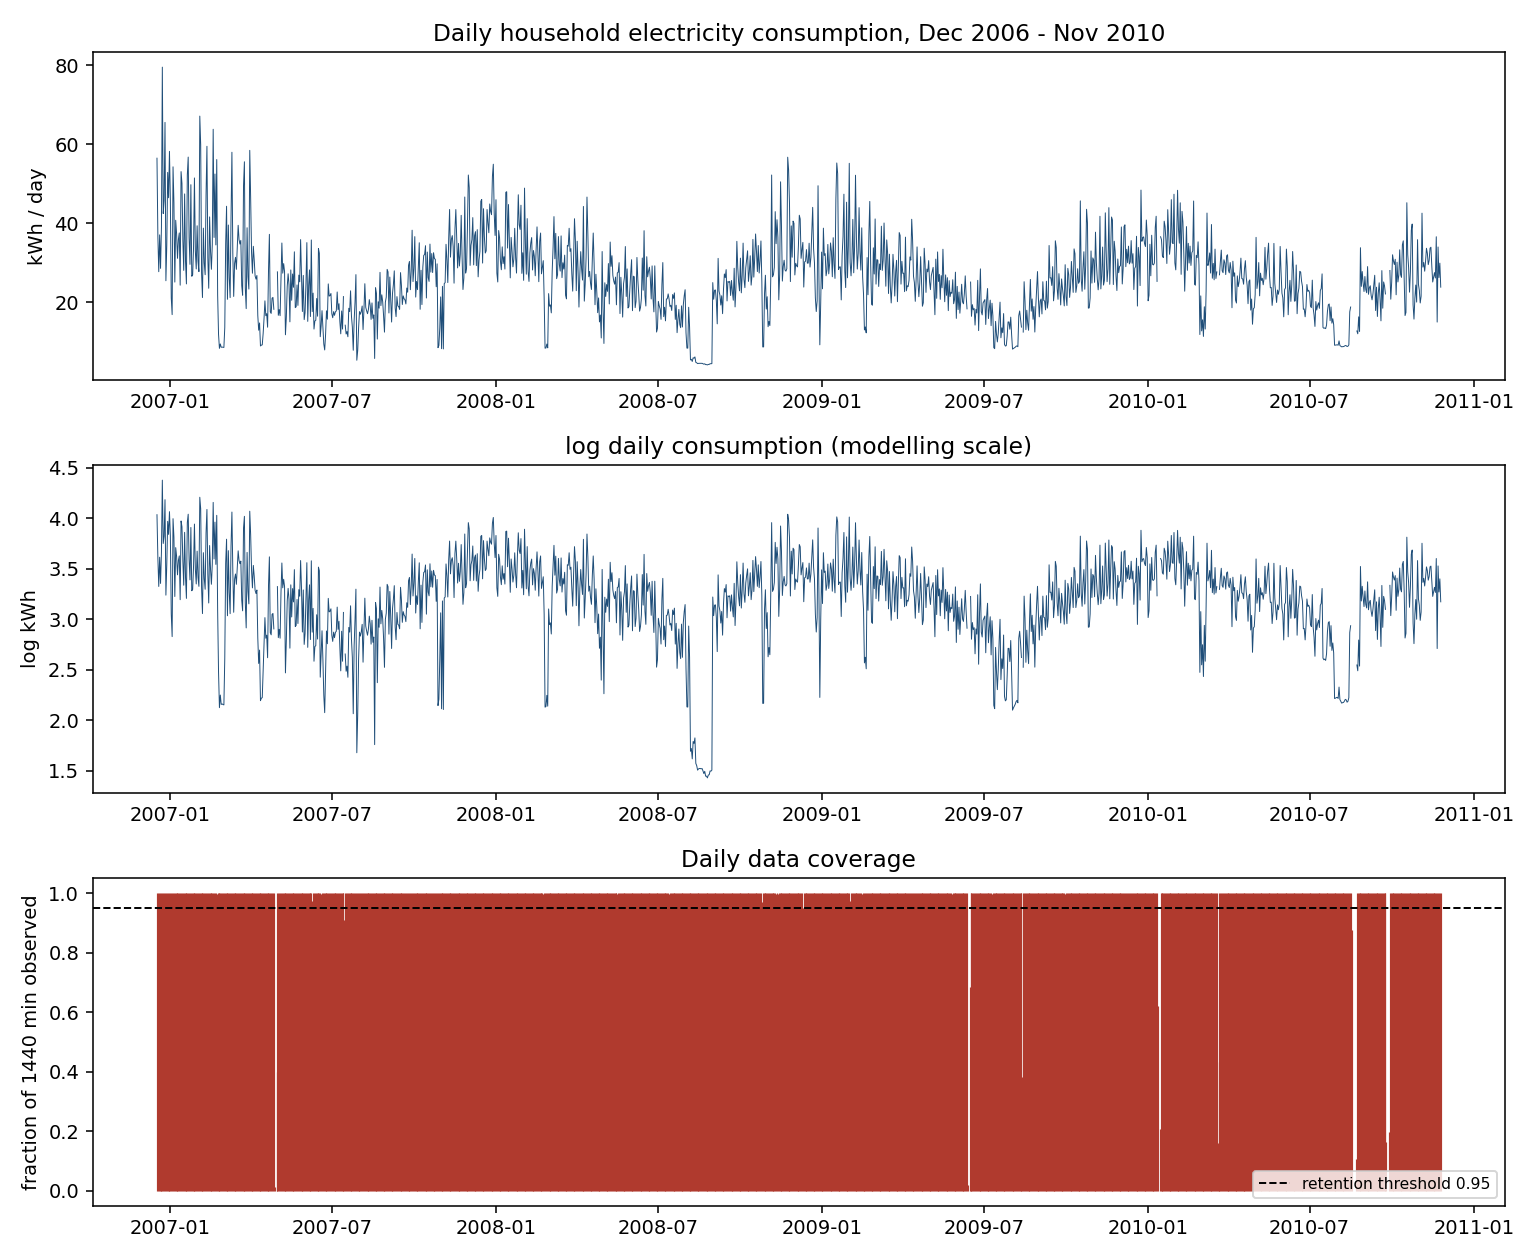
\includegraphics[width=\textwidth]{figures/01_series_and_coverage.png}
\caption{The daily series on both scales, and daily data coverage against the
95\% retention threshold. The contiguous nature of the gaps is visible in the
bottom panel; the deep summer troughs in the top panel are real absences, not
missing data.}
\end{figure}

\section{Exploratory analysis that determined the model}

Rather than assert a specification, three pre-fits were used to choose one. All
use ordinary least squares on the same mean structure (intercept, linear trend,
two harmonics, day-of-week) and examine the residuals.

\subsection{Response scale: the log transform is the wrong default}

\begin{center}
\small
\begin{tabular}{@{}lrrrrr@{}}
\toprule
Scale & $R^2$ & Residual skew & Residual kurtosis & Heterosced.\ $p$ & $\hat\rho_1$ \\
\midrule
$y$ (kWh)     & 0.452 & $\phantom{-}0.059$ & 5.00 & $<0.0001$ & 0.368 \\
$\sqrt{y}$    & 0.445 & $-0.699$ & 4.57 & $0.0239$ & 0.469 \\
$\log y$      & 0.410 & $-1.450$ & 6.18 & $<0.0001$ & 0.583 \\
\bottomrule
\end{tabular}
\end{center}

The conventional argument for logging a positive, right-skewed response fails
here. Raw daily kWh, once season and day-of-week are removed, is
\emph{already} symmetric (skew $0.059$). Taking logs overcorrects badly
(skew $-1.450$), because the multi-week absence periods --- August 2008 sits at
$4.76\kwh$/day for 25 consecutive days --- become extreme \emph{left} outliers
on the log scale. The transform creates the asymmetry it was meant to remove.
Gaussian kurtosis is $3$; every scale is well above it, which is the argument
for a $t$ likelihood regardless of scale.

\subsection{Error memory: how much, and is it real?}

The residual autocorrelation function decays far more slowly than AR(1)
implies. The observed values at lags $1$, $2$ and $3$ are $0.582$, $0.455$ and
$0.432$, and lag $7$ is still $0.273$ --- where an AR(1) with
$\rho_1 = 0.582$ would predict only $0.023$. Taken at face value this argues
for AR(3) or higher.

It should not be taken at face value. Repeating the exercise with the four
sustained absence blocks removed changes the answer completely:

\begin{center}
\small
\begin{tabular}{@{}lcccc@{}}
\toprule
Sample & BIC-preferred order & $\hat\phi_1$ & $\hat\sigma_\eta$ & marginal sd / one-step sd \\
\midrule
All observed days & $p=3$ & $0.453$ & $0.270$ & $1.25$ \\
Absence blocks excluded & $p=1$ & $0.380$ & $0.258$ & $1.09$ \\
\bottomrule
\end{tabular}
\end{center}

The apparent long memory is largely a \emph{regime} effect: a three-week
absence looks like enormous persistence to an autocorrelation function. The
right response is not a higher-order AR but AR(1) for genuine weather
persistence plus a heavy-tailed innovation to absorb the blocks --- a
conclusion the out-of-sample comparison later confirms.

The four blocks are: 24 Feb--2 Mar 2007 (7 days, mean $9.18\kwh$);
6--30 Aug 2008 (25 days, $4.76\kwh$); 1--8 Aug 2009 (8 days, $9.01\kwh$);
and 29 Jul--14 Aug 2010 (17 days, $9.09\kwh$).

\begin{figure}[htbp]
\centering
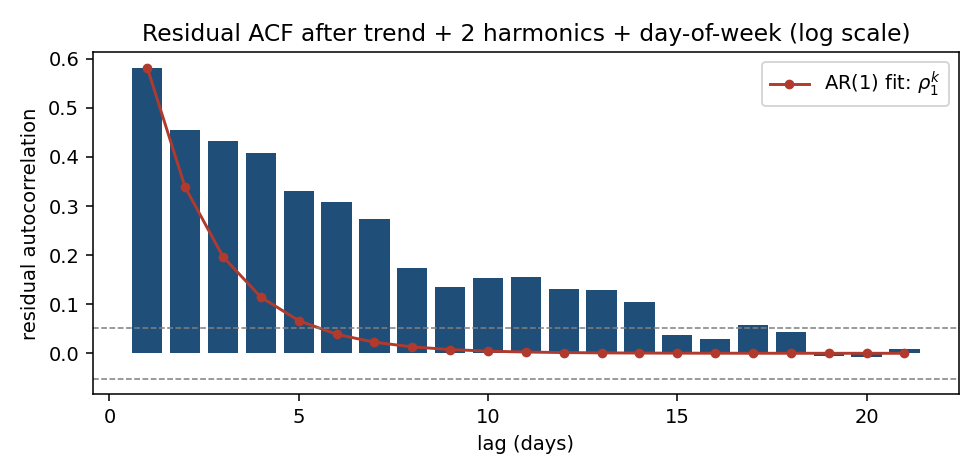
\includegraphics[width=0.62\textwidth]{figures/01b_residual_acf.png}
\caption{Residual autocorrelation after trend, two harmonics, and day-of-week,
against the geometric decay an AR(1) would produce. The gap at lags 3--10 is
what the absence blocks contribute.}
\end{figure}

\section{The model}

\subsection{Specification}

Let $y_t$ denote daily consumption in kWh on a gap-free daily grid
$t = 1,\dots,T$ with $T = 1440$, and let $z_t = g(y_t)$ for a link $g$ that is
either the identity or the logarithm (the choice is treated as a modelling
decision to be tested, not assumed). Then
\begin{align}
z_t &= \mathbf{x}_t^{\top}\boldsymbol\beta + \varepsilon_t, \label{eq:mean}\\
\mathbf{x}_t^{\top}\boldsymbol\beta
 &= \beta_0
  + \beta_1 \frac{t - \bar t}{365}
  + \sum_{j=1}^{J}\left[a_j \sin\frac{2\pi j t}{365} + b_j \cos\frac{2\pi j t}{365}\right]
  + \sum_{k=2}^{7}\delta_k \mathbf{1}\{\mathrm{dow}_t = k\}, \label{eq:design}\\
\varepsilon_t &= \sum_{\ell=1}^{p}\phi_\ell\,\varepsilon_{t-\ell} + \eta_t,
\qquad
\eta_t \sim t_\nu(0,\sigma^2). \label{eq:ar}
\end{align}
Monday is the baseline day, so $\delta_k$ measures the deviation of day $k$
from Monday; the reported weekly profile is re-centred on the weekly mean.
The trend is centred at $\bar t$, which decorrelates it from the intercept and
makes $\beta_0$ the level at the midpoint of the record. The harmonics use
raw $t$, as mandated.

Three features of \eqref{eq:ar} are deliberate and each earns its place in
Section~\ref{sec:compare}.

\paragraph{The AR term is what makes Q5 answerable.} For an AR(1), the $h$-step
predictive standard deviation is
$\sigma\sqrt{\sum_{j<h}\phi^{2j}}$, rising from $\sigma$ at $h=1$ toward the
stationary limit $\sigma/\sqrt{1-\phi^2}$. The ratio of those two numbers
\emph{is} the answer to ``how does uncertainty change with the horizon''. With
independent errors the ratio is $1$ and the question is vacuous.

\paragraph{Heavy tails absorb the absence regime.} With Gaussian innovations,
the four absence blocks inflate $\sigma$ and blur every other inference. The
$t_\nu$ innovation lets the model treat them as outliers rather than as
evidence about typical variability.

\paragraph{The error process lives on the full calendar grid.} $\varepsilon_t$
is defined for all $t$, but the likelihood is evaluated only on observed days.
The $23$ missing days are thus \emph{imputed} as part of inference rather than
dropped, which both preserves the AR structure across gaps and propagates the
uncertainty about those days into everything else.

\subsection{Priors}

Priors are weakly informative and scaled to the response, which matters because
the same code fits both the log scale (coefficients of order $0.1$) and the kWh
scale (coefficients of order $10$).

\begin{center}
\small
\begin{tabular}{@{}p{0.14\textwidth}p{0.36\textwidth}p{0.42\textwidth}@{}}
\toprule
Parameter & Prior & Rationale \\
\midrule
$\beta_0$ & $N(0,\tau_0^2)$, $\tau_0 = 5$ (log) or $100$ (kWh)
  & Generous relative to a level of $3.2$ or $26$ \\
other $\beta$ & $N(0,\tau^2)$, $\tau = 2$ (log) or $40$ (kWh)
  & Admits effects far larger than any plausible one \\
$\sigma$ & half-$t(3, 0, A)$, $A = 1$ (log) or $20$ (kWh)
  & Gelman's recommendation: heavy-tailed, proper, no spike at $0$ \\
$\phi$ & Uniform on the stationary region
  & Non-informative but excludes non-stationary forecasts \\
$\nu - 2$ & Exponential, mean $10$
  & Keeps the variance finite ($\nu>2$) while allowing near-Gaussian tails \\
$z_t$, $t$ missing & Implied by \eqref{eq:ar}
  & Imputation, not deletion \\
\bottomrule
\end{tabular}
\end{center}

The half-$t$ prior on $\sigma$ is implemented through the standard
inverse-gamma auxiliary variable: if
$\sigma^2\mid\xi \sim \mathrm{IG}(\nu_\sigma/2,\ \nu_\sigma/(2\xi))$ and
$\xi \sim \mathrm{IG}(1/2,\ 1/A^2)$, then $\sigma \sim$ half-$t(\nu_\sigma,0,A)$
and both steps stay conjugate.

\section{Algorithms and techniques}

\subsection{Why a hand-written sampler}

No probabilistic programming language was available in the environment (no
JAGS, Stan, PyMC, or R), so the sampler was written from scratch in
\code{numpy}/\code{scipy}. This turned out to be an advantage rather than a
constraint: the model is conditionally conjugate in almost every block, so a
Gibbs sampler with two Metropolis steps mixes better than generic HMC would on
the $1{,}440$-dimensional latent error path, and it runs a four-chain,
$40{,}000$-iteration fit in about 44 seconds.

\subsection{The $t$ distribution as a scale mixture}

The key device is to write the $t_\nu$ innovation as a continuous mixture of
normals,
\begin{equation}
\eta_t \mid \lambda_t \sim N\!\left(0,\ \sigma^2/\lambda_t\right),
\qquad
\lambda_t \sim \mathrm{Gamma}(\nu/2,\ \nu/2),
\end{equation}
so that marginalising $\lambda_t$ recovers $\eta_t \sim t_\nu(0,\sigma^2)$.
Conditional on $\boldsymbol\lambda$ the model is a weighted Gaussian
regression, which restores conjugacy for $\boldsymbol\beta$ and $\sigma^2$.
The $\lambda_t$ have a second, interpretive use: a small posterior mean
$\lambda_t$ marks a day the likelihood had to downweight.

\subsection{Full conditionals}

Write $\tilde{\mathbf{x}}_t = \mathbf{x}_t - \sum_\ell \phi_\ell \mathbf{x}_{t-\ell}$
and $\tilde z_t = z_t - \sum_\ell \phi_\ell z_{t-\ell}$ for the quasi-differenced
data, and let $w_t = \lambda_t/\sigma^2$.

\paragraph{$\boldsymbol\beta$ (Gibbs, conjugate normal).} Exactly
\[
\boldsymbol\beta \mid \cdot \ \sim\ N\!\left(\mathbf{Q}^{-1}\mathbf{r},\ \mathbf{Q}^{-1}\right),
\quad
\mathbf{Q} = \boldsymbol\Sigma_0^{-1}
 + \sum_{t>p} w_t \tilde{\mathbf{x}}_t\tilde{\mathbf{x}}_t^{\top}
 + \mathbf{X}_{1:p}^{\top}\mathbf{V}_0^{-1}\mathbf{X}_{1:p},
\]
with $\mathbf{r}$ the matching linear term. The third piece is the contribution
of the first $p$ days, drawn from the \emph{exact} stationary distribution
$\mathbf{V}_0$ of the AR($p$) rather than conditioned away, so the chain starts
stationary and no warm-up of the error process is required. For $p=1$,
$\mathbf{V}_0 = \sigma^2/(1-\phi^2)$; for $p=2$ it is obtained by solving the
discrete Lyapunov equation $\mathbf{V} = \mathbf{A}\mathbf{V}\mathbf{A}^{\top}+\mathbf{Q}$
in companion form.

\paragraph{$\sigma^2$ and $\xi$ (Gibbs, inverse-gamma).}
$\sigma^2 \mid \cdot \sim \mathrm{IG}\big((\nu_\sigma + T)/2,\ \nu_\sigma/(2\xi) + S/2\big)$
where $S = \sum_{t>p}\lambda_t\eta_t^2 + \boldsymbol\varepsilon_{1:p}^{\top}\mathbf{V}_0^{-1}\boldsymbol\varepsilon_{1:p}\sigma^2$,
followed by
$\xi \mid \sigma^2 \sim \mathrm{IG}\big((\nu_\sigma+1)/2,\ A^{-2} + \nu_\sigma/\sigma^2\big)$.

\paragraph{$\lambda_t$ (Gibbs, gamma).}
$\lambda_t \mid \cdot \sim \mathrm{Gamma}\big((\nu+1)/2,\ (\nu + \eta_t^2/\sigma^2)/2\big)$,
vectorised across all $t$.

\paragraph{$\nu$ (Metropolis, random walk on $\log(\nu-2)$).} The conditional
depends on the data only through $\boldsymbol\lambda$, giving the gamma
likelihood $\prod_t \mathrm{Gamma}(\lambda_t;\nu/2,\nu/2)$; the Jacobian
$\log(\nu-2)$ is included in the acceptance ratio.

\paragraph{$\boldsymbol\phi$ (Metropolis, random walk).} The conditional is
Gaussian in $\boldsymbol\phi$ multiplied by the stationary-initialisation factor
\[
|\mathbf{V}_0|^{-1/2}\exp\!\left\{-\tfrac12\boldsymbol\varepsilon_{1:p}^{\top}\mathbf{V}_0^{-1}\boldsymbol\varepsilon_{1:p}\right\},
\]
which is not conjugate. Proposals outside the stationary region are rejected
outright by checking that the companion matrix has spectral radius below one.

\paragraph{Missing $z_t$ (Gibbs, normal).} The log conditional is quadratic in
$\varepsilon_t$, so its exact mean and precision are read off the gradient and
curvature of $\sum_s \lambda_s\eta_s^2$ with respect to $\varepsilon_t$,
accounting for the $p+1$ terms in which $\varepsilon_t$ appears.

Both random-walk step sizes are adapted during burn-in toward a $30\%$
acceptance rate and then held fixed, so the sampled portion of the chain uses a
time-homogeneous kernel.

\subsection{Convergence diagnostics}

Rank-normalised split-$\hat R$ and bulk effective sample size were implemented
directly, following Vehtari et al.: draws are rank-normalised through the
inverse normal CDF, each chain is split in half to expose within-chain drift,
and ESS uses Geyer's initial positive sequence to truncate the autocorrelation
sum. Targets were $\hat R < 1.01$ and ESS $> 400$ for every parameter.

\subsection{Validation against simulated data}

A sampler that has not been tested against known truth cannot be trusted. Data
were simulated from the model itself with known $\boldsymbol\beta$, $\phi$,
$\sigma$, and $\nu$, and with missing days blanked in contiguous blocks to mimic
the real pattern. Result: $14$ of $15$ parameters had the true value inside the
$95\%$ credible interval (the miss was $\delta_{\text{Tue}}$, truth $0.060$
against an interval ending at $0.059$), worst $\hat R = 1.014$, minimum bulk
ESS $317$. Recovery of $\phi$ was essentially exact: truth $0.450$, posterior
mean $0.449$, interval $[0.406, 0.492]$.

\subsection{Model comparison machinery}
\label{sec:compare}

\paragraph{WAIC.} Computed from pointwise log predictive densities using the
one-step-ahead conditional factorisation $\sum_t \log p(y_t \mid y_{<t},\theta)$.
Two details make the comparison valid. First, models with different AR orders
would otherwise use different numbers of terms, so a \emph{single shared index
set} is used throughout: the $1{,}399$ days that are observed and whose two
preceding days are also observed. Second, log-scale models carry the Jacobian
$-\log y_t$, so every log-likelihood is a density of daily kWh and models on
different response scales are directly comparable.

\paragraph{Held-out forecasting, two designs.} WAIC scores one-step-ahead fit,
which is the wrong target for a forecasting question, so every modelling
decision was re-tested out of sample. Models were refitted on data through
30 Nov 2009 ($1{,}072$ observed days) and never saw the final twelve months
($345$ observed days).

\begin{itemize}
\item \textbf{Design A --- single origin.} A twelve-month forecast from
30 Nov 2009. This is the honest ``what could you have said a year in advance''
test and it produces the fan chart and coverage table. Its weakness is that the
$361$ horizons come from one realisation, so horizon-by-horizon scores are
correlated.
\item \textbf{Design B --- rolling origin.} Horizons $1$--$60$ from origins
spread through the holdout year. Parameters still come only from the training
period, but each forecast conditions on actuals up to its own origin. Crucially
this requires \emph{no refitting}: given $\boldsymbol\beta$, the error at any
day with an observed response is simply $\varepsilon_t = z_t - \mathbf{x}_t^{\top}\boldsymbol\beta$.
With roughly $113$ origins per horizon, the accuracy-versus-horizon curve gains
real replication.
\end{itemize}

\paragraph{Scoring rules.} Three, because they probe different things.
\emph{Log predictive density} rewards sharp, well-located densities and
punishes overconfidence severely. \emph{CRPS} is computed with the exact
ensemble identity
$\mathrm{CRPS} = \frac{1}{N}\sum_i|x_i - y| - \frac{1}{N^2}\sum_{i<j}|x_i-x_j|$,
evaluated in $O(N\log N)$ by sorting; it is in kWh and so is interpretable.
\emph{Empirical coverage} of central $50\%$ and $95\%$ intervals, plus PIT
histograms, tests calibration directly.

One refinement is worth noting. The $h$-step predictive density is not
available in closed form, but it need not be estimated by kernel smoothing:
conditional on a posterior draw and the simulated path up to $h-1$, the final
innovation is exactly $t_\nu$. Marginalising only that last step gives the
Rao-Blackwellised mixture
\begin{equation}
p(y_{T+h}\mid \mathbf{y}) \approx \frac{1}{S}\sum_{s=1}^{S}
 t_{\nu^{(s)}}\!\left(z_{T+h};\ \mu^{(s)}_{T+h} + \textstyle\sum_\ell \phi^{(s)}_\ell \varepsilon^{(s)}_{T+h-\ell},\ \sigma^{(s)}\right),
\end{equation}
which is far more accurate than smoothing a predictive sample and costs nothing
extra.

\section{Results}

\subsection{Convergence and the fitted family}

Seven specifications were fitted to the full series, all sharing priors, data,
and likelihood index. Four chains of $40{,}000$ iterations, $10{,}000$
discarded, thinned by $5$, giving $24{,}000$ draws. Diagnostics passed
throughout: worst $\hat R$ across all seven models was $1.011$ and the minimum
bulk ESS was $399$ (both in M2, for $\nu$, the hardest parameter); the
headline model M7 had worst $\hat R = 1.007$ and minimum ESS $1{,}072$.

\begin{center}
\small
\begin{tabular}{@{}llrrrl@{}}
\toprule
ID & Specification & $\mathrm{elpd}_{\mathrm{WAIC}}$ & $p_{\mathrm{WAIC}}$ & $\Delta$ & Purpose \\
\midrule
M5 & $J{=}2$, AR(2)$+t$, log & $-4594.0$ & 18.1 & $0.0$ & longer error memory? \\
M4 & $J{=}3$, AR(1)$+t$, log & $-4613.2$ & 19.4 & $-19.2$ & third harmonic too far? \\
M3 & $J{=}2$, AR(1)$+t$, log & $-4622.3$ & 17.2 & $-28.4$ & adds harmonic 2 \\
M2 & $J{=}1$, AR(1)$+t$, log & $-4636.2$ & 15.3 & $-42.3$ & mandated starting point \\
M7 & $J{=}2$, AR(1)$+t$, kWh & $-4656.8$ & 16.0 & $-62.9$ & isolates the log transform \\
M6 & $J{=}2$, AR(1)$+$Gauss, log & $-4657.6$ & 16.0 & $-63.7$ & isolates heavy tails \\
M1 & $J{=}1$, iid Gaussian, log & $-5006.8$ & 12.6 & $-412.9$ & naive baseline \\
\bottomrule
\end{tabular}
\end{center}

\subsection{WAIC and the holdout disagree, and the holdout wins}

Each modelling decision was isolated as a paired comparison under both
criteria. Design B differences are per-day mean log predictive densities with
paired standard errors.

\begin{center}
\small
\begin{tabular}{@{}lrlrl@{}}
\toprule
Decision & WAIC $\Delta$elpd & verdict & Holdout $\Delta$lpd/day & verdict \\
\midrule
AR(1)$+t$ vs iid Gaussian     & $+370.6 \pm 36.3$ & supported   & $+0.0139 \pm 0.0016$ & supported \\
Second harmonic ($J{=}2$ vs $1$) & $+13.9 \pm 5.7$  & supported   & $+0.0366 \pm 0.0035$ & supported \\
Third harmonic ($J{=}3$ vs $2$)  & $+9.1 \pm 4.5$   & supported   & $+0.0457 \pm 0.0017$ & supported \\
$t$ vs Gaussian, given AR(1)  & $+35.3 \pm 11.9$  & supported   & $+0.0094 \pm 0.0011$ & supported \\
AR(2) vs AR(1)                & $+28.4 \pm 10.6$  & \textbf{supported} & $\mathbf{-0.0232 \pm 0.0011}$ & \textbf{rejected} \\
Log scale vs kWh scale        & $+34.5 \pm 17.7$  & inconclusive & $\mathbf{-0.0772 \pm 0.0040}$ & \textbf{kWh wins} \\
\bottomrule
\end{tabular}
\end{center}

The two rows in bold are the substantive surprises. WAIC favours AR(2) by
nearly three standard errors, yet AR(2) forecasts \emph{worse} out of sample by
more than twenty. The explanation is the one the exploratory analysis
anticipated: the extra lag is fitting the absence blocks, which improves
one-step-ahead in-sample density but does not generalise. Likewise the log
transform, which WAIC cannot decide about, is clearly harmful for forecasting.
Accordingly the headline model is \textbf{M7}: $J{=}2$, AR(1) with $t$
innovations, on the kWh scale.

\subsection{Answers to the six questions}

All figures below are posterior means with $95\%$ credible intervals from M7.

\paragraph{Q1 --- variation over the study period.} Mean consumption is
$25.96\kwh$/day $[25.41, 26.50]$ at the record midpoint. The annual cycle is by
far the largest source of variation, with a full seasonal range of
$18.25\kwh$/day $[16.48, 20.06]$; the weekly cycle contributes about
$4.56\kwh$; the one-step innovation standard deviation is $5.59\kwh$.

\paragraph{Q2 --- long-term trend: no evidence.} The slope is
$-0.186\kwh$/year $[-0.667, +0.292]$, equivalently $-0.72\%$/year
$[-2.57, +1.13]$. The interval straddles zero and
$\Pr(\text{slope}<0\mid\text{data}) = 0.775$ --- suggestive of a mild decline,
far from conclusive. Over the whole record the implied change is
$-0.74\kwh$/day $[-2.63, +1.15]$, i.e. under $3\%$ of the mean level. The
honest answer is that four years is too short to separate a small trend from
the annual cycle, particularly since the record is $3$ years $11$ months rather
than a whole number of years.

\paragraph{Q3 --- annual seasonality, and yes the second harmonic matters.}
The first harmonic has amplitude $8.08\kwh$ $[7.31, 8.85]$, a peak-to-trough
swing of $16.15\kwh$, and peaks on \textbf{14 January} $[9\text{--}20$ Jan$]$.
The second harmonic has amplitude $2.43\kwh$ $[1.68, 3.19]$, giving an
amplitude ratio $A_2/A_1 = 0.302$ $[0.204, 0.405]$ with
$\Pr(A_2 > 0.15\,A_1 \mid \text{data}) = 0.999$. Three independent lines of
evidence therefore agree that harmonic 2 is important: the amplitude ratio, the
WAIC difference ($+13.9 \pm 5.7$), and the held-out log score
($+0.0366 \pm 0.0035$). Substantively, the second harmonic makes the annual
curve \emph{asymmetric} --- it deepens and delays the summer trough while
sharpening the winter peak, which is what a heating-dominated load with a long
flat summer floor actually looks like. The third harmonic helps too, by an even
larger held-out margin, which is the strongest hint that two harmonics still
under-fit the seasonal shape.

\begin{figure}[htbp]
\centering
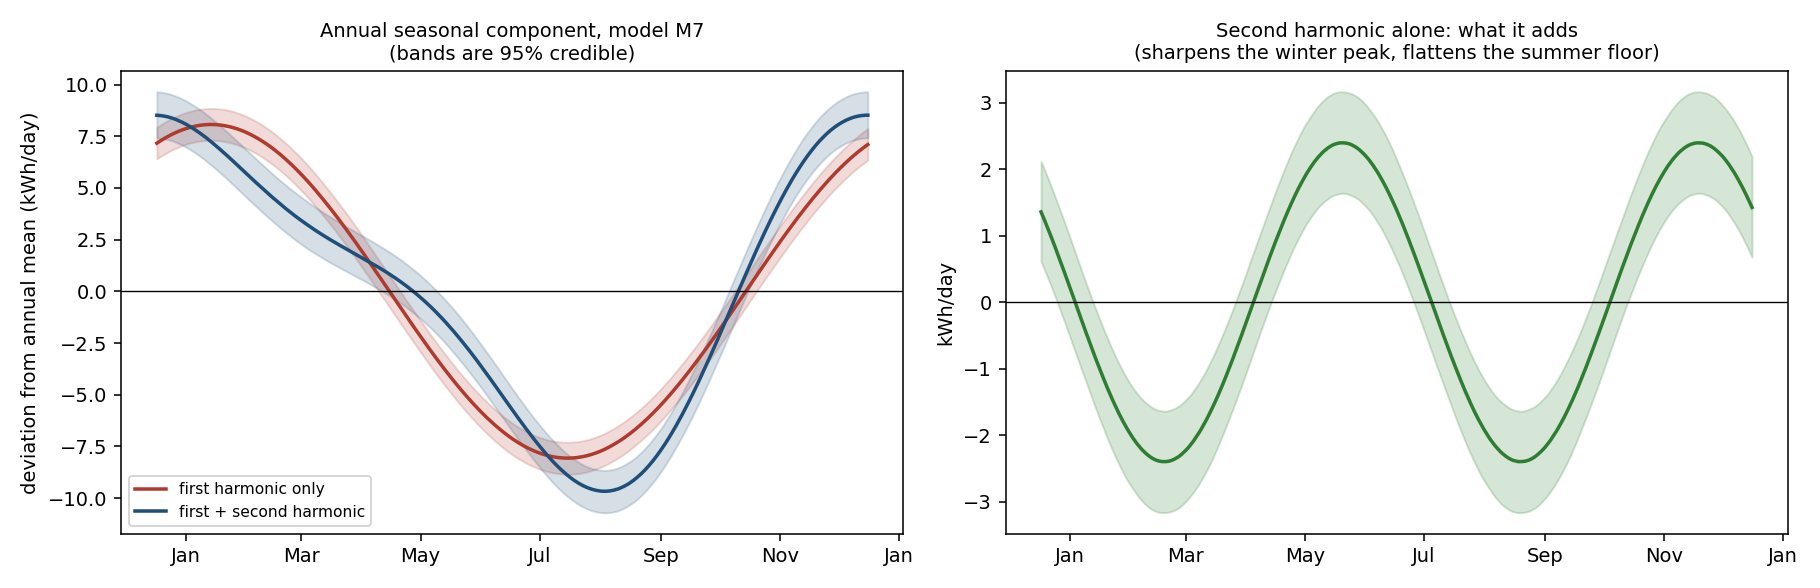
\includegraphics[width=\textwidth]{figures/05_seasonal.png}
\caption{Left: the annual seasonal component with one harmonic (red) and two
(blue). Adding the second harmonic deepens the summer trough by roughly
$1.5\kwh$/day and shifts it later. Right: the second harmonic in isolation.}
\end{figure}

\paragraph{Q4 --- weekly pattern: strong and unambiguous.} Deviations from the
weekly mean, in kWh/day: Saturday $+3.50$ $[2.67, 4.33]$, Sunday $+3.02$
$[2.21, 3.85]$, Wednesday $-0.10$, Tuesday $-0.41$, Friday $-1.12$, Monday
$-2.15$, Thursday $-2.75$ $[-3.51, -1.99]$. The weekend-minus-weekday contrast
is $4.56\kwh$/day $[3.71, 5.42]$ with
$\Pr(\text{weekend} > \text{weekday} \mid \text{data}) = 1.0000$ --- the
clearest effect in the entire analysis, and physically obvious: the house is
occupied.

\paragraph{Q5 --- predictive accuracy saturates within four days.} This is the
cleanest result. The width of the $95\%$ predictive interval rises from
$28.9\kwh$ at one day ahead to $31.4\kwh$ by day seven and then stops, sitting
at $31.2\kwh$ even sixty days out --- a total increase of $8\%$. The empirical
curve matches the AR($p$) theoretical prediction $\sqrt{\sum_{j<h}\psi_j^2}$
almost exactly, and its ceiling is the stationary ratio
$1/\sqrt{1-\phi^2} = 1.079$ $[1.057, 1.105]$ implied by
$\phi = 0.375$ $[0.323, 0.426]$. Calibration holds up: $95\%$ intervals cover
$94.5\%$ at $h=1$ and $95.2\%$ at $h=7$.

The interpretable conclusion is blunt. Knowing yesterday's consumption buys
about $8\%$ narrower intervals, and only for three or four days. Beyond roughly
a week, a forecast of this household's demand is seasonal-plus-weekly
climatology and nothing more.

\begin{figure}[htbp]
\centering
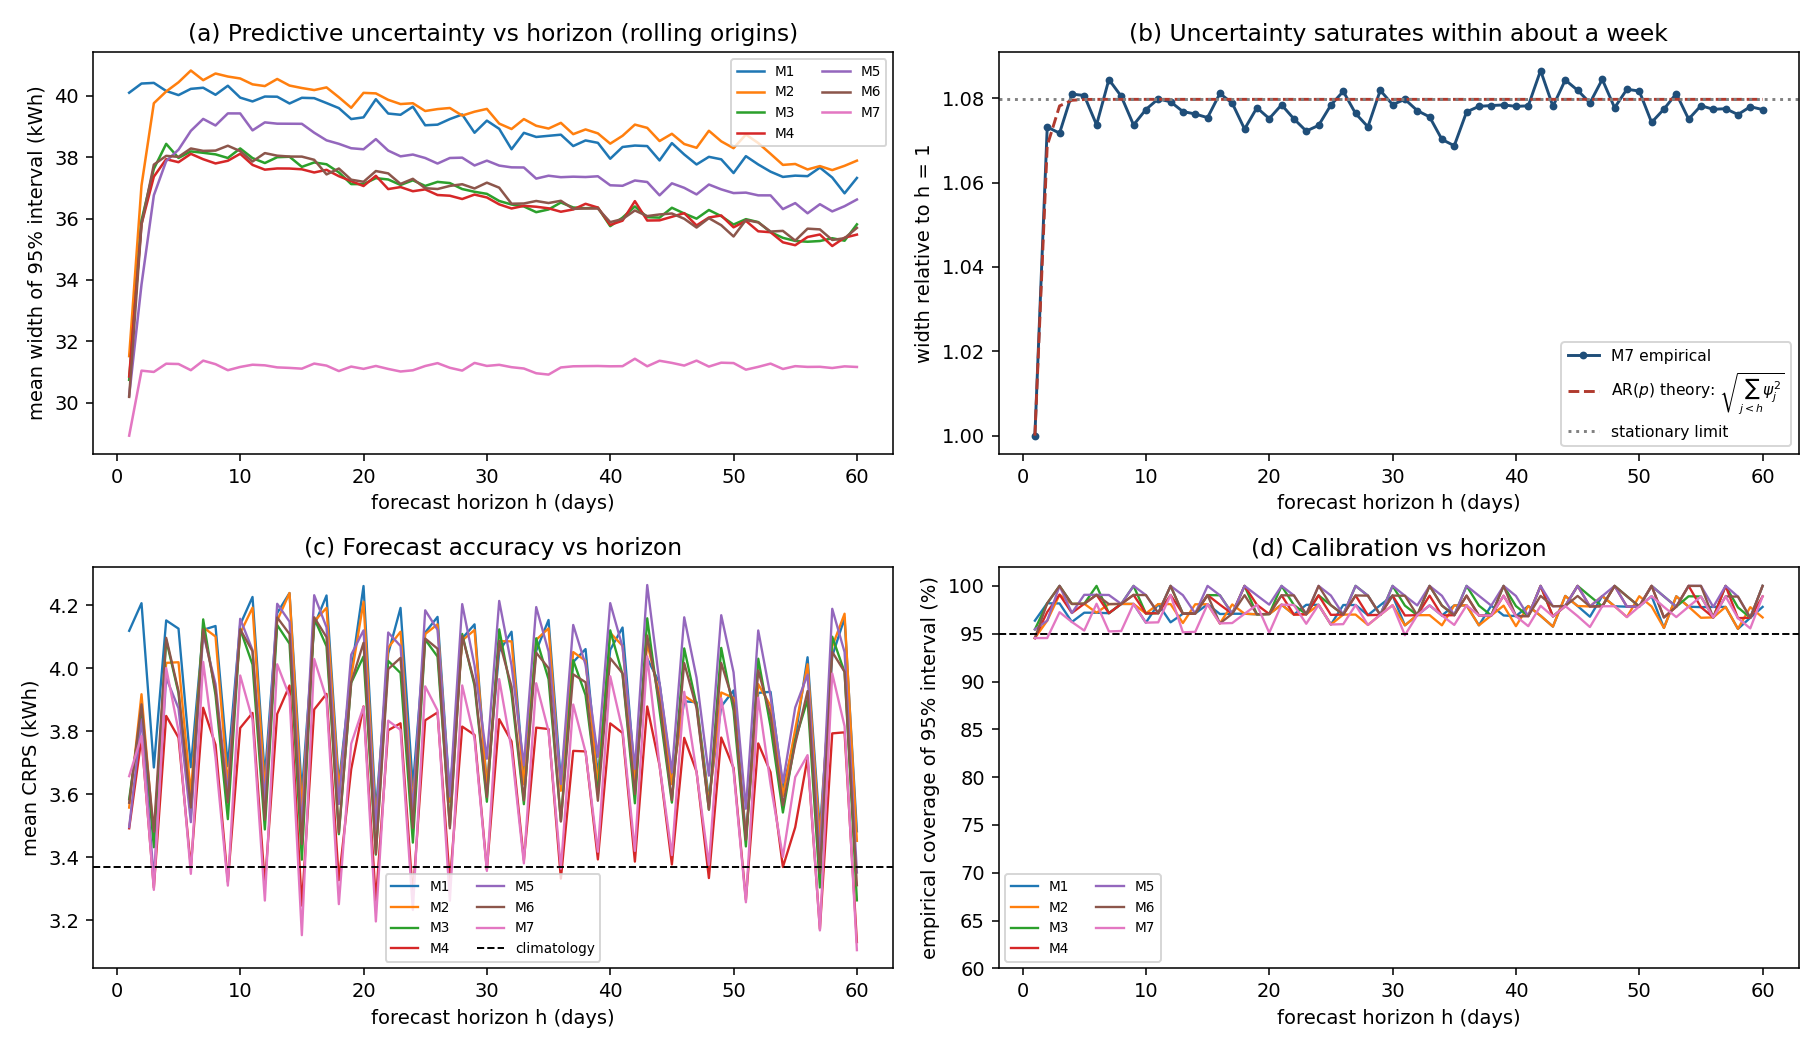
\includegraphics[width=\textwidth]{figures/04_horizon.png}
\caption{Predictive uncertainty, accuracy, and calibration against forecast
horizon. Panel (b) is the answer to Q5: uncertainty saturates by day four and
tracks AR(1) theory exactly. The sawtooth in panel (c) is an artefact of
origins spaced three days apart, discussed in Section~\ref{sec:roadblocks}.}
\end{figure}

\paragraph{Q6 --- unusual periods.} Two diagnostics are needed, for a reason
that is itself a finding. One-step-ahead posterior predictive $p$-values
$p_t = \Pr(y_t^{\text{rep}} \le y_t \mid \mathbf{y})$ flag $31$ of $1{,}408$
days at the $1\%$ level, mostly \emph{high} days ($23$ against $8$ low, where
$14$ of each is expected), concentrated in the first winter: 23 Dec 2006
($79.6$ against $38.2\kwh$ fitted, $z = +7.1$), 3 Feb 2007 ($67.2$ vs $35.3$),
18 Feb 2007 ($63.8$ vs $33.6$). That asymmetry says the model systematically
under-predicts extreme winter peaks.

But a one-step-ahead check \emph{cannot} detect a sustained anomaly: once the
AR(1) term absorbs a drop, the model expects the low level to continue and
subsequent innovations look normal. Since Q6 asks about \emph{periods}, the
test statistic must be a block statistic --- here the mean of a rolling
$14$-day window, referred to its posterior predictive distribution under the
stationary error process. Of $1{,}416$ windows, $63$ fall below $p = 0.01$ and
$19$ rise above $p = 0.99$. Those windows overlap heavily, so the effective
number of independent windows is nearer $1416/14 \approx 101$; even against
that denominator, $82$ flagged windows is far more than the $2$ expected under
a correctly specified model. Sustained departures are thus a systematic
feature, not sampling noise. Merging overlapping same-direction runs yields
thirteen distinct episodes.

\begin{center}
\small
\begin{tabular}{@{}llrrrrr@{}}
\toprule
From & To & Days & Observed & Expected & Ratio & $p$ \\
\midrule
17 Dec 2006 & 6 Jan 2007 & 21 & 42.16 & 34.57 & 1.22 & 0.001 \\
2 Feb 2007 & 25 Feb 2007 & 24 & 36.84 & 31.14 & 1.18 & 0.001 \\
21 Feb 2007 & 11 Mar 2007 & 19 & 25.10 & 29.79 & 0.84 & $<$0.001 \\
19 Mar 2007 & 7 Apr 2007 & 20 & 33.54 & 27.94 & 1.20 & 0.003 \\
3 Apr 2007 & 28 Apr 2007 & 26 & 19.99 & 27.01 & 0.74 & $<$0.001 \\
21 Oct 2007 & 11 Nov 2007 & 22 & 25.12 & 30.50 & 0.82 & 0.001 \\
19 Dec 2007 & 2 Jan 2008 & 15 & 40.89 & 34.44 & 1.19 & 0.008 \\
17 Feb 2008 & 9 Mar 2008 & 22 & 24.95 & 29.78 & 0.84 & 0.001 \\
\textbf{1 Aug 2008} & \textbf{5 Sep 2008} & \textbf{36} & \textbf{8.55} & \textbf{17.21} & \textbf{0.50} & \textbf{$<$0.001} \\
21 Oct 2008 & 9 Nov 2008 & 20 & 25.31 & 30.29 & 0.84 & 0.003 \\
27 Jan 2010 & 10 Feb 2010 & 15 & 37.85 & 31.15 & 1.21 & 0.007 \\
22 Feb 2010 & 8 Mar 2010 & 15 & 23.19 & 28.94 & 0.80 & 0.007 \\
\textbf{1 Aug 2010} & \textbf{15 Aug 2010} & \textbf{15} & \textbf{9.64} & \textbf{16.30} & \textbf{0.59} & \textbf{0.009} \\
\bottomrule
\end{tabular}

\end{center}

\noindent\emph{Observed} and \emph{Expected} are mean kWh/day over the episode,
the latter from the fitted systematic component; $p$ is the smaller tail
probability of the most extreme $14$-day window in the episode. The thirteen
episodes are generated directly into this table by
\code{05\_derived.py}, so no figures here are transcribed by hand.

The August episodes are the signature of French summer holidays: in August 2008
the house ran at \emph{half} the consumption the seasonal model expects for
five straight weeks, which is a base load with nobody home. The winter episodes
run the other way and are almost certainly cold snaps. Both kinds are
behavioural or meteorological, and neither is predictable from a calendar ---
which is precisely the argument for the $t$ likelihood, and precisely the
limitation named in Section~\ref{sec:limits}.

\begin{figure}[htbp]
\centering
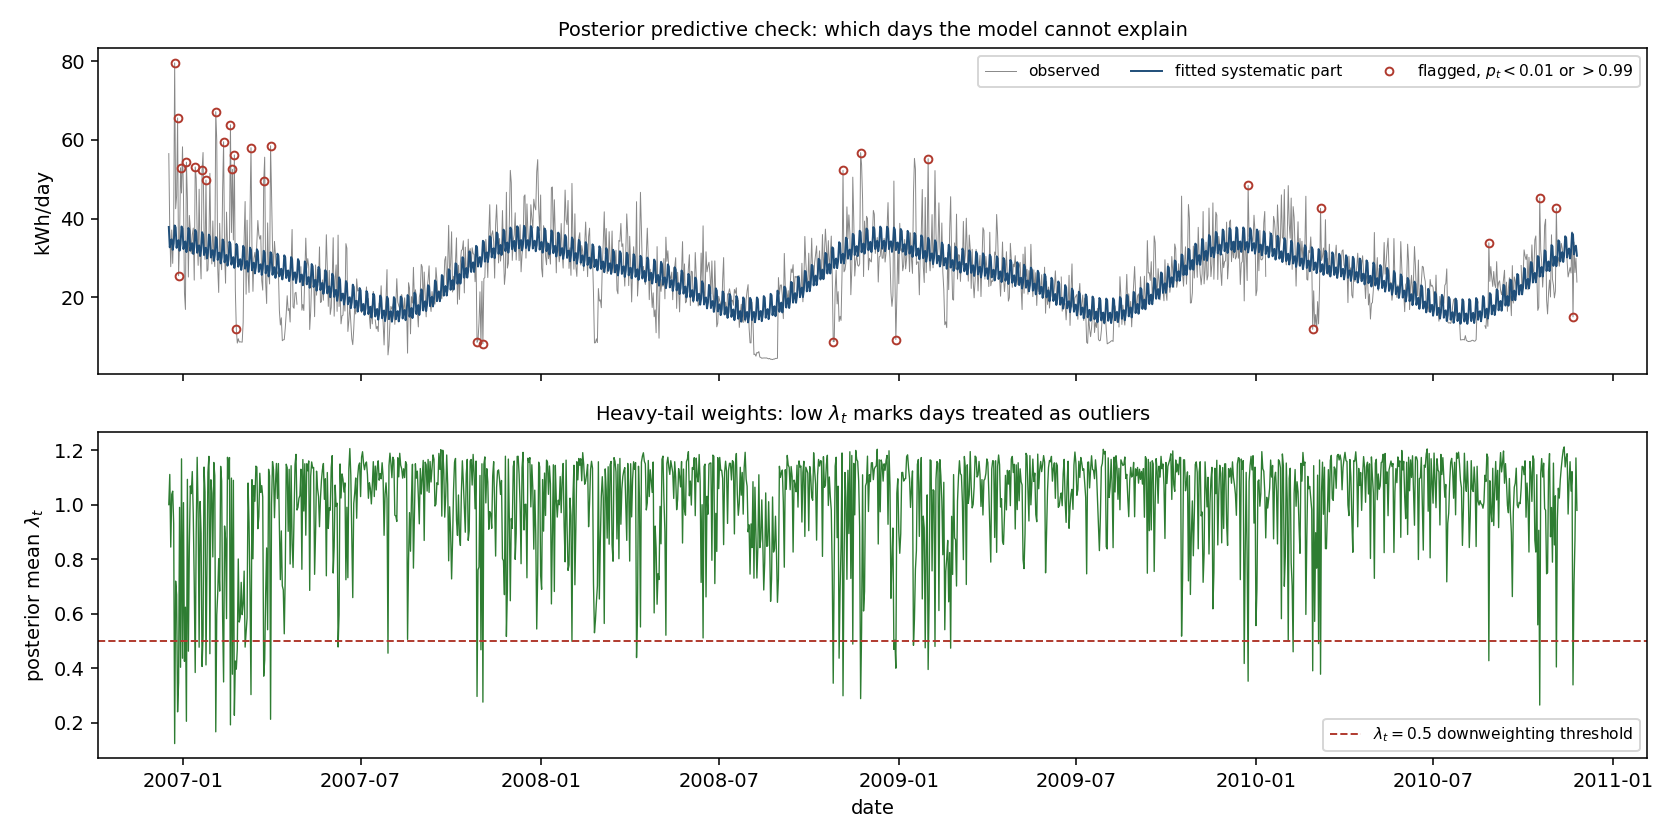
\includegraphics[width=\textwidth]{figures/05_anomalies.png}
\caption{Top: fitted systematic component against observed consumption, with
one-step-ahead flagged days circled. Bottom: posterior mean heavy-tail weights
$\lambda_t$; low values mark days the likelihood downweighted.}
\end{figure}

\section{Roadblocks}
\label{sec:roadblocks}

\subsection{Data engineering}

\begin{enumerate}[leftmargin=*]
\item \textbf{Silent parse corruption.} The \code{?} missing-value code and the
day-first dates each fail quietly rather than loudly. Both were handled
explicitly, and the sub-meter-versus-total inequality was used as an
independent check that parsing was correct ($0$ violations).

\item \textbf{Power versus energy.} \code{Global\_active\_power} is kW, not kWh.
The division by $60$ in \eqref{eq:agg} is easy to omit and produces a series
wrong by a factor of $24$ while still looking entirely plausible.

\item \textbf{Contiguous missingness creating phantom anomalies.} Because gaps
arrive in runs, a naive daily sum turns partially observed days into dramatic
low-consumption events, which Q6 would then faithfully report as findings. The
$95\%$ coverage rule removes $23$ days; without it, several would have
contaminated the anomaly table.
\end{enumerate}

\subsection{Modelling decisions that came out backwards}

\begin{enumerate}[leftmargin=*,start=4]
\item \textbf{The log transform was the wrong default, and I had recommended
it.} The initial plan specified a log-scale response on the usual grounds that
daily kWh is positive and right-skewed. The residual diagnostics contradicted
this (skew $+0.059$ on the kWh scale against $-1.450$ on the log scale) and the
holdout confirmed it decisively ($-0.077$ nats/day). The cause is specific to
this dataset: logging converts the multi-week absence periods from moderate
low values into extreme left-tail outliers. Keeping the scale as an explicitly
tested decision rather than an assumption is what caught this.

\item \textbf{Apparent long error memory was a regime artefact.} The residual
ACF at lag 7 is $+0.273$ where AR(1) predicts $+0.023$, and BIC on all days
prefers AR(3). Excluding the absence blocks, BIC prefers AR(1) and $\hat\phi_1$
drops from $0.58$ to $0.38$. Fitting the apparent memory with extra AR lags
would have been fitting four holidays.

\item \textbf{WAIC and held-out forecasting disagreed on AR(2).} WAIC favoured
it by $+28.4 \pm 10.6$; the holdout rejected it by $-0.0232 \pm 0.0011$ per
day. WAIC on a one-step-ahead conditional factorisation is a weak proxy for
forecast skill, and information criteria are known to be unreliable for
autocorrelated series. This is why the holdout, not WAIC, is the criterion
defended here.
\end{enumerate}

\subsection{Implementation and evaluation bugs}

\begin{enumerate}[leftmargin=*,start=7]
\item \textbf{Non-comparable WAIC across AR orders.} Models with $p = 0, 1, 2$
naturally evaluate $1{,}417$, $1{,}408$, and $1{,}399$ pointwise terms. Summing
different numbers of terms and comparing the totals is meaningless. Fixed by
forcing one shared likelihood index set across the whole family. The analogous
problem across response scales was fixed with the log-Jacobian.

\item \textbf{Misaligned rolling-origin comparison.} Each model initially chose
its own valid origins based on its own lag requirements, so paired differences
compared forecasts of different calendar days --- and crashed on a shape
mismatch, which is the good outcome. Fixed by computing one origin set from the
strictest requirement in the family and asserting that every model scores
identical target days at every horizon.

\item \textbf{Dependent horizons in the rolling design.} Origins spaced three
days apart mean horizons $h$ and $h+3$ score nearly the same calendar dates, so
adjacent horizons are not independent samples and the accuracy curve oscillates
(the sawtooth in Figure 4c). Verified not to be a misalignment bug by checking
that the weekday composition is flat across horizons (weekend fraction $0.25$
to $0.30$). The fix --- stepping origins every day and scoring all horizons on
one common date set --- is identified but not yet applied.

\item \textbf{A formatting bug that made CRPS look $100\times$ too large.}
Coverage columns were detected with \code{key.startswith("c")}, which also
matches \code{"crps"}, so CRPS was multiplied by $100$ in one table. Harmless
to the analysis, but a good illustration of why the same quantity was reported
in two places.

\item \textbf{One-step-ahead diagnostics cannot answer Q6.} The first anomaly
check used sustained runs of low $\lambda_t$ and found exactly one four-day
run, which is wrong --- the 36-day August 2008 absence was invisible. The
reason is structural: after the AR(1) term adapts, a sustained anomaly produces
normal-sized innovations. Q6 required a block-level posterior predictive check
with a window-mean test statistic, which then recovered all the expected
episodes.

\item \textbf{Spurious numerical warnings.} \code{numpy} on macOS reported
divide-by-zero, overflow, and invalid-value warnings from every \code{matmul}.
Confirmed spurious by checking a matrix with condition number $1.52$ that
raised all four flags while returning exactly correct finite results: Apple's
Accelerate BLAS sets IEEE status bits inside its SIMD kernels. Suppressed with
a documented filter rather than left to mask real problems.
\end{enumerate}

\subsection{Open problem: climatology still wins at long horizons}

The one unresolved issue, stated plainly because it qualifies every long-range
claim above. A reference forecast built from nothing but day-of-year means
(a $\pm 7$-day window, split by weekend/weekday, from the training years only)
\emph{beats every fitted model} on the twelve-month-ahead test:

\begin{center}
\small
\begin{tabular}{@{}lrrr@{}}
\toprule
Forecast & mean lpd & CRPS (kWh) & mean $95\%$ width (kWh) \\
\midrule
Day-of-year climatology & $\mathbf{-3.225}$ & $\mathbf{3.371}$ & $29.89$ \\
M7 ($J{=}2$, AR(1)$+t$, kWh) & $-3.311$ & $3.666$ & $31.25$ \\
M4 ($J{=}3$, AR(1)$+t$, log) & $-3.365$ & $3.683$ & $38.08$ \\
M3 ($J{=}2$, AR(1)$+t$, log) & $-3.413$ & $3.904$ & $38.47$ \\
M1 ($J{=}1$, iid Gaussian, log) & $-3.453$ & $3.959$ & $40.56$ \\
\bottomrule
\end{tabular}
\end{center}

The climatology is both sharper and more accurate. The working diagnosis is
that two harmonics cannot reproduce the true annual shape --- in particular the
sharp August trough --- so the unexplained seasonal structure inflates $\sigma$,
widening intervals on every ordinary day. Three pieces of evidence support this
reading: each added harmonic keeps improving the held-out score (harmonic 3
helps \emph{more} than harmonic 2); the log-scale models are visibly
over-dispersed ($50\%$ intervals covering $58$--$68\%$); and the climatology's
advantage comes precisely from being locally flexible in day-of-year while
carrying no extrapolated trend.

The planned resolution is to extend the harmonic order to $J = 6$ on the kWh
scale, fit a variant without the linear trend (whose extrapolation over a year
may itself be damaging), and enter the climatology as a competitor in the
rolling design rather than only the single-origin one. Until that is done, the
long-horizon forecasts here should be read as a lower bound on achievable
accuracy.

\section{Limitations}
\label{sec:limits}

\begin{enumerate}[leftmargin=*]
\item \textbf{One house, not a market.} A single household's daily load has no
averaging across consumers to smooth individual behaviour --- one person
deciding to do laundry moves the response. Conclusions describe \emph{this}
household, and the wide predictive intervals ($\pm 15\kwh$ around a mean of
$26\kwh$) are a genuine feature, not a modelling failure.

\item \textbf{No temperature covariate.} Heating and hot water drive most of the
seasonal signal, and heating demand responds to weather, not to the calendar.
The harmonics are a proxy for \emph{average} weather on a given day of year, so
a cold snap in a mild February is unexplained noise by construction. This is
the honest explanation for most of the Q6 anomaly table and the main reason the
$t$ likelihood is doing real work. Merging in daily temperature for Paris would
be the single highest-value extension.

\item \textbf{Trend and season are mildly confounded.} The record spans $3$
years $11$ months, not a whole number of years, so the seasonal cycle is not
perfectly balanced across the trend. This widens the trend interval and is part
of why Q2 is inconclusive.

\item \textbf{The mandated period is $365$, not $365.25$ days.} Over a
four-year record this drifts by about three days. The brief mandates $365$ and
that is what is used, but the phase estimates carry this small systematic
error.

\item \textbf{The absence regime is modelled as outliers, not as structure.}
A latent two-state occupancy process (home/away) would explain the blocks
rather than merely downweighting them, and would likely fix the long-horizon
deficit. It is a substantially larger model and was left as an extension.

\item \textbf{WAIC uses a conditional factorisation.} Comparing
$\sum_t \log p(y_t \mid \text{past})$ across models with different AR orders
compares different factorisations of the joint density. The shared index set
makes the arithmetic valid, but the holdout remains the criterion to trust.
\end{enumerate}

\section{Reproducing the analysis}

Everything runs on \code{numpy}, \code{scipy}, \code{pandas}, and
\code{matplotlib}; no probabilistic programming language is required. Scripts
execute in order.

\begin{center}
\small
\begin{tabular}{@{}lll@{}}
\toprule
Script & Purpose & Runtime \\
\midrule
\code{01\_aggregate.py} & Parse, aggregate to daily kWh, coverage rule & 11\,s \\
\code{01b\_transform\_check.py} & Response-scale and error-structure evidence & 13\,s \\
\code{01c\_ar\_order\_check.py} & AR order, with and without absence blocks & 1\,s \\
\code{02\_validate\_sampler.py} & Recovery of known parameters on simulated data & 11\,s \\
\code{03\_fit\_models.py} & Fit M1--M7, convergence, WAIC & 6\,min \\
\code{04\_holdout.py} & Refit on training data, designs A and B, scoring & 4\,min \\
\code{05\_derived.py} & Derived posteriors, anomaly checks, answer figures & 5\,s \\
\bottomrule
\end{tabular}
\end{center}

\code{model.py} holds the sampler, diagnostics, WAIC, forecasting, and scoring
rules. Results are written as plain text to \code{results/} and figures to
\code{figures/}, so every number quoted above is traceable to a file.

\vspace{6pt}
\noindent\textbf{Data source.} UCI Machine Learning Repository, Individual
Household Electric Power Consumption,
\url{https://archive.ics.uci.edu/dataset/235/}.

\end{document}
